% ==============================================================================
% This file is part of the "LaTeX template for writing the Final Degree Work
% report". It has been developed to aid the students of the Bachelor's Degree in
% Video Game Design and Development at the Jaume I University.
%
% (c) 2019 Sergio Barrachina Mir and José Vte. Martí Avilés
%
% The template can be used and distributed under the next license:
%  Creative Commons Attribution-NonCommercial-ShareAlike (CC BY-NC-SA)
%  http://creativecommons.org/licenses/by-nc-sa/3.0/
%  http://creativecommons.org/licenses/by-nc-sa/3.0/legalcode
%
% Atom editor configuration follows:
% !TEX root = ./report.tex
% !TeX spellcheck = en-US
% ==============================================================================

\chapter{System Analysis and Design}

\minitoc{}

\bigskip{}

In this sections, we will detail which requirements must be acomplished to consider that the neural network solves its task correctly. Also, we will specify the system used to develop this work and its minimum specifications.

\section{Requirement Analysis}

\subsection{Functional Requirements}

The following must be fulfilled to provide a realistic imitation:

\begin{itemize}
 \item The neural network will be able to play indepently the game
 \item The network will receive as input what is seeing
 \item The network will receive as input immediate past actions and images
 \item The network will output the action made (continuous actions)
 \item The network will output the probability of performing an action (discrete actions)
 \item The network will adapt its actions to reaction times of who is imitating
 \item The network and the real player would not be differentiated when playing
\end{itemize}

%======================================================================
% Comando para que todos los requisitos funcionales tengan el mismo
% formato
%----------------------------------------------------------------------
\newcommand{\functionalrequirement}[5]{
 \begin{table}[htbp]
  \centering
  \begin{tabular}{lp{.7\linewidth}}              \toprule
   Input:  & #3                         \\ \midrule
   Output: & #4                         \\ \midrule
   \multicolumn{2}{p{.9\linewidth}}{#5} \\ \bottomrule
  \end{tabular}
  \caption{Functional requirement «#2»}
  \label{#1}
 \end{table}
}
%======================================================================

%\functionalrequirement%
%{tab:cred1} % label
%{CRED1. Credits query} % name
%{Available credits query} % input
%{User credits} % output
%{Each user has a number of credits. When the user requests information
% about the number of credits he owns, this value must be returned. } % description

%\functionalrequirement%
%{tab:cred2} % label
%{CRED2. Credits purchase} % name
%{Number of credits to purchase} % input
%{Transaction result: correct or failed} % output
%{The user requests the purchase of a given number of credits. An attempt is made to make the corresponding charge in the payment method previously selected by the user. If the payment is correctly made, the number of credits of the user is increased and he/she is notified that the operation has been correctly carried out. If there is a failure in the collection process, the user is informed of the error.} % description


\subsection{Non-functional Requirements}

\begin{itemize}
 \item The network will be scalable to more complex problems
 \item The network will be decently trained in reasonable time
 \item The network will be sample efficient when training
\end{itemize}


\section{System Design}
\label{sec:system_design}

To train an agent, an environment is needed. The training is executed in a game build, where the custom bot plays the game and the neural network tries to guess its moves. After trained, the neural network can be fed into the Agent class and play the game by itself in the editor. The Figure~\ref{fig:classes} shows the class diagram of the environment:
\begin{figure}[b]
  \centering
		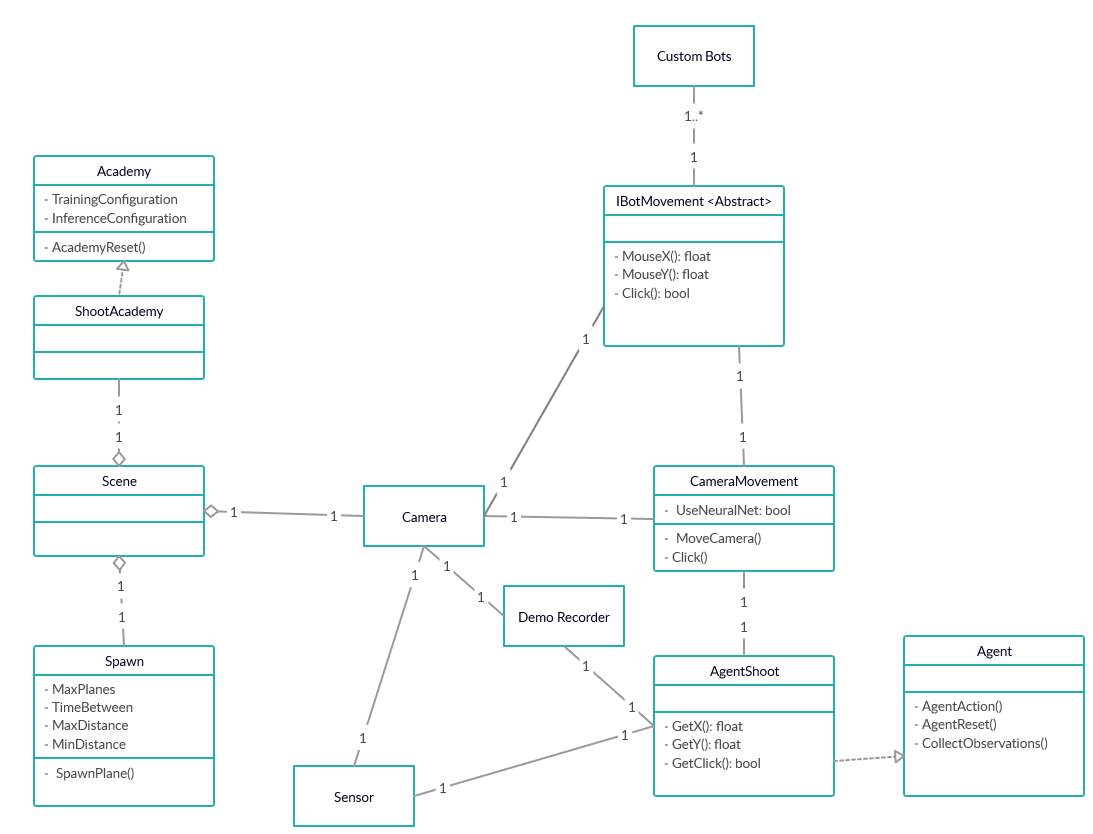
\includegraphics[width=.8\textwidth]{img/classDiagram.png}
  \caption{Class diagram of the training environment}
  \label{fig:classes}
\end{figure}

The scene has one custom Academy (ShootAcademy), a Camera and a Spawner that creates the enemies randomly in execution time. The camera contains one custom bot (the abstract class allows to create new bots and test them without changing references), a movement handler (CameraMovement) which handles the moves made by the bot or the neural network, a custom Agent that generates and executes trained neural networks, a visual sensor and a Demo Recorder (when activated, it generates a dataset for Imitation learning).

The classes Academy, Agent, DemoRecorder and Sensor are provided by the ML Agents SDK~\cite{mlagents}.

\section{System Architecture}

\begin{figure}[h]
  \centering
		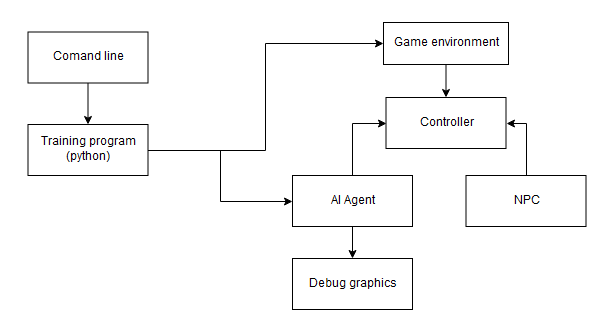
\includegraphics[width=.8\textwidth]{img/systemArchitecture.png}
  \caption{Diagram of the system architecture}
  \label{fig:architecture}
\end{figure}

ML Agents works using an environment in Unity to train neural networks. The networks are trained in a python program (executed using the command line) that communicates with that environment. In the environment, there will be a controller that allows either the NPC or the trained agent to play the game. A graph will be displayed in the UI to see live how well the agent is performing.

\section{Interface Design}

To acknowledge how well is the neural net adapting to the bot movement, the guesses of the bot are displayed in a real time graph alongside the bot's real move. There is also a centered sight to better see how the bot behaves. Figure~\ref{fig:uicomp} shows a complete game window while training.

The graph displays 3 main lines (see Figure~\ref{fig:uigraph}): the red one is the move made by the bot, the blue and green ones are the highest and lowest guess of the bot (since the bot's movements are not perfect, these two lines can vary from being almost touching to being really wide). Other 3 lines in the back display the weighted average move and its standard deviation.

The image at the bottom left is what the neural network receives as input. It helps verify that everything works correctly (Figure ~\ref{fig:uivision}): if the agent action and the NPC action look similar, then it's very likely that the agent would perform well~\footnote{Even though sometimes the agent can look like the NPC that imitates during training, when playing it can behave differently depending on the observations it receives. In section ~\ref{sec:movememory} there is an example on why this phenomenon can happen. }.
\begin{figure}[h]
  \centering
		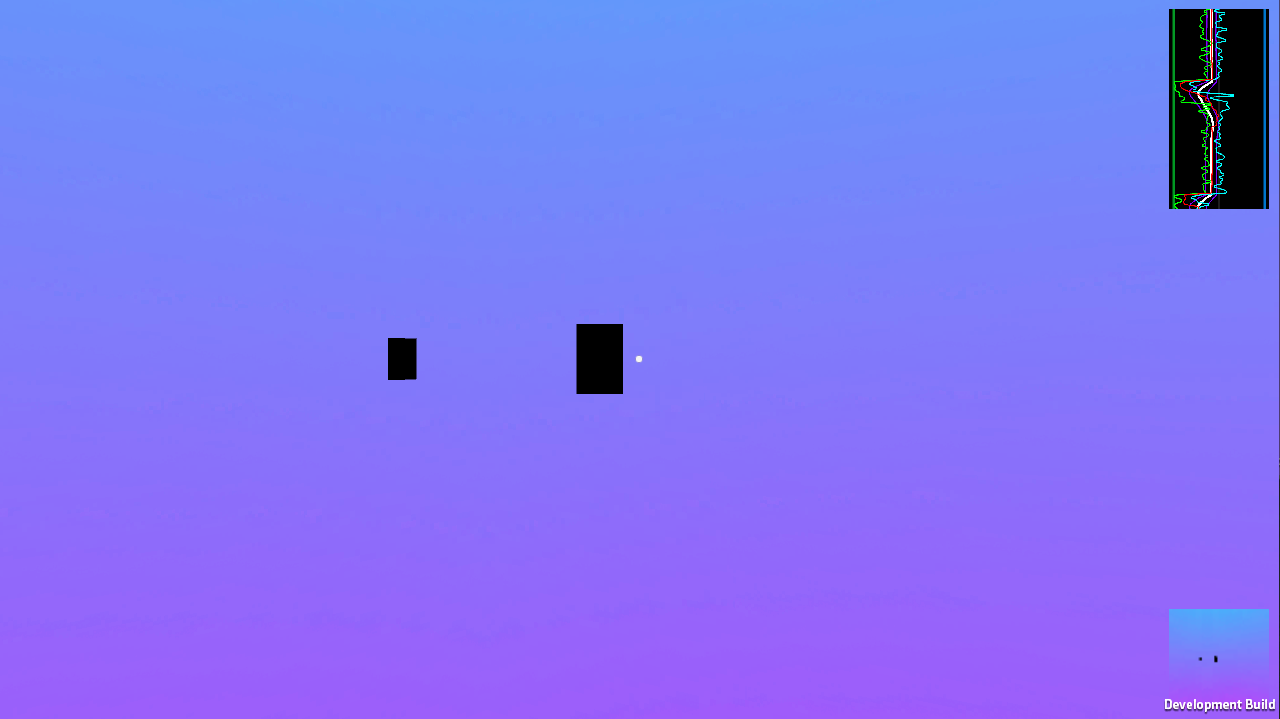
\includegraphics[width=.9\textwidth]{img/uiComplete.png}
  \caption{Complete screen of the game}
  \label{fig:uicomp}
\end{figure}

\begin{figure}[h]
    \centering
    \begin{subfigure}[h]{0.3\textwidth}
        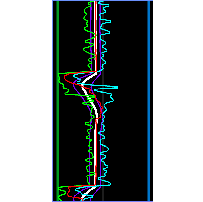
\includegraphics[width=\textwidth]{img/uiGraph.png}
        \caption{Move Graph}
        \label{fig:uigraph}
    \end{subfigure}
    ~ %add desired spacing between images, e. g. ~, \quad, \qquad, \hfill etc. 
      %(or a blank line to force the subfigure onto a new line)
    \begin{subfigure}[h]{0.3\textwidth}
        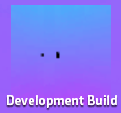
\includegraphics[width=\textwidth]{img/uiVision.png}
        \caption{Input Vision}
        \label{fig:uivision}
    \end{subfigure}
		\caption{Debugging UI elements}
\end{figure}

%\begin{figure}
%\begin{center}
%    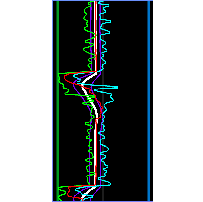
\includegraphics[width=0.3\textwidth]{img/uiGraph.png}
%
%    \hspace{1cm}
%
%    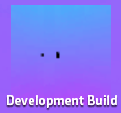
\includegraphics[width=0.3\textwidth]{img/uiVision.png}
%   \vspace{0.1cm}
%    \caption{UI elements: graph and vision}
%    \label{fig:uielem}
%  \end{center}
%\end{figure}

